\documentclass[a4paper, 11pt]{article}

\usepackage{parskip}
\usepackage{fontspec}
\usepackage{cite}
\usepackage{hyperref}
\usepackage[nonumberlist, acronym]{glossaries}
\usepackage{xcolor}
\usepackage[margin=2cm]{geometry}
\usepackage{graphicx}
\usepackage{array}
\usepackage{mfirstuc}
\usepackage[official]{eurosym}
\usepackage{minted}
\usepackage{caption}

\graphicspath{{./images/}}

\setmonofont{Courier New}
\definecolor{bg}{rgb}{0.85, 0.85, 0.85}
\setmintedinline{bgcolor=bg}
\setminted{bgcolor=bg, linenos}
\renewcommand{\theFancyVerbLine}{\small\arabic{FancyVerbLine}}
\captionsetup[table]{skip=10pt}
\captionsetup[figure]{skip=10pt}
\captionsetup[listing]{skip=10pt}
\setacronymstyle{long-short}

\makeglossaries

\title{A title}

\begin{document}
    \maketitle
    
    \begin{abstract}
    some abstract
    \end{abstract}
    \clearpage

    \tableofcontents
    \clearpage
    
    \newacronym
        {MD}
        {MD}
        {Markdown}
    \newacronym
        {OOP}
        {OOP}
        {Object Oriented Programming}

    \newglossaryentry{function}
    {
        name=function,
        description={An operation which has an input and output}
    }

    \newglossaryentry{variable}
    {
        name=variable,
        description={A symbol which can take on any value in a defined domain}
    }

    \section{A header}
    \label{sec:my-header}

    \section{Another header}
    \label{another-header}

    Referencing previous section as Section \ref{sec:my-header}

    \subsection{A subheader}
    \label{a-subheader}

    Mentioning a \gls{function} and a \gls{variable}.

    Mentioning the acronym \gls{OOP}, and the acronym \gls{MD}.

    Mentioning the acronym \gls{OOP} a second time, fully abbreviated.

    This is some text with \textit{light emphasis}. This is some text
    with \textbf{strong emphasis}.

    This is some code \mintinline{text}{x = 3}.

    A block of python code, referenced by Listing
    \ref{lst:python-code-example}

    \begin{listing}[H]
        \begin{minted}[mathescape, gobble=12, linenos={true}]{python}
            def f(x):
                return x**2
            
            if __name__=="__main__":
                x = 3
                y = f(x)
                print(y)
        \end{minted}
        \caption{An example of python code}
        \label{lst:python-code-example}
    \end{listing}

    A block of .NET code, referenced by Listing
    \ref{lst:dotnet-code-example}

    \begin{listing}[H]
        \begin{minted}[mathescape, gobble=12, linenos={true}]{cs}
            using System;
            
            class Program
            {
                static void Main(string[] args)
                {
                    Console.WriteLine("Hello");
                }
            }
        \end{minted}
        \caption{An example of dotnet code}
        \label{lst:dotnet-code-example}
    \end{listing}

    An example of a listing imported from an external file. Line
    \ref{ln:print-statement} contains a \mintinline{text}{print}
    statement:

    \begin{listing}[H]
        \inputminted
            [
                mathescape,
                firstline={4},
                lastline={8},
                linenos={true}
            ]
            {python}
            {imported-code-block.py}
        \caption{A block of code imported from an external file}
        \label{lst:imported-code-block}
    \end{listing}

    A command line block, without line numbers or highlighting,

    \begin{listing}[H]
        \begin{minted}[mathescape, gobble=12, linenos={False}]{text}
            PS> get-childitem -recurse .
        \end{minted}
        \caption{A command line block}
        \label{lst:command-line-block}
    \end{listing}

    A bulleted list:

    \begin{itemize}
        \item item
        \begin{itemize}
            \item subitem
            \item subitem
            \item subitem
        \end{itemize}
        \item item
    \end{itemize}

    An ordered list:

    \begin{enumerate}
        \item item
        \begin{enumerate}
            \item subitem
            \item subitem
            \item subitem
        \end{enumerate}
        \item item
    \end{enumerate}

    A figure, referenced by Figure \ref{fig:banana}

    \begin{figure}[H]
        \centering
        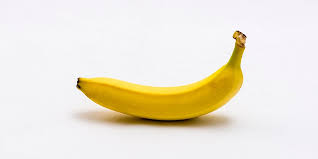
\includegraphics[scale=1.0]{banana.jpg}
        \caption{A banana}
        \label{fig:banana}
    \end{figure}

    A simple table, referenced by Table \ref{tab:my-simple-table}

    \begin{table}[h]
        \caption{Simple table caption}
        \label{tab:my-simple-table}
        \centering
        \begin{tabular}{|c|c|c|c|}
            \hline
            \bfseries{Right} &
            \bfseries{Left} &
            \bfseries{Center} &
            \bfseries{Default} \\
            \hline
            12 &
            12 &
            12 &
            12 \\
            \hline
            123 &
            123 &
            123 &
            123 \\
            \hline
            1 &
            1 &
            1 &
            1 \\
            \hline
        \end{tabular}
    \end{table}

    A grid table, referenced by Table \ref{tab:my-grid-table}

    \begin{table}[h]
        \caption{Grid table caption}
        \label{tab:my-grid-table}
        \centering
        \begin{tabular}{|p{\dimexpr0.22\textwidth-2\tabcolsep}|p{\dimexpr0.22\textwidth-2\tabcolsep}|p{\dimexpr0.29\textwidth-2\tabcolsep}|}
            \hline
            \bfseries{Fruit} &
            \bfseries{Price} &
            \bfseries{Advantages} \\
            \hline
            Bananas &
            1.34 &
            
    \begin{itemize}
        \item built-in wrapper
        \item bright color
    \end{itemize} \\
            \hline
            Oranges &
            2.10 &
            
    \begin{itemize}
        \item cures scurvy
        \item tasty
    \end{itemize} \\
            \hline
        \end{tabular}
    \end{table}

    \begin{table}[h]
        \caption{Simple table caption, with explicit column widths}
        \label{tab:my-simple-table-explicit}
        \centering
        \begin{tabular}{|p{2cm}|p{1cm}|c|c|}
            \hline
            \bfseries{Right} &
            \bfseries{Left} &
            \bfseries{Center} &
            \bfseries{Default} \\
            \hline
            12 &
            12 &
            12 &
            12 \\
            \hline
            123 &
            123 &
            123 &
            123 \\
            \hline
            1 &
            1 &
            1 &
            1 \\
            \hline
        \end{tabular}
    \end{table}

    A \mintinline{text}{plantuml} class diagram, referenced by Figure
    \ref{fig:plantuml-diagram}:

    \begin{figure}[H]
        \centering
        \includegraphics[scale=0.8]{images/plantuml-diagram.png}
        \caption{A class diagram}
        \label{fig:plantuml-diagram}
    \end{figure}

    A \mintinline{text}{graphviz} graph, referenced by Figure
    \ref{fig:graphviz-diagram}.

    \begin{figure}[H]
        \centering
        \includegraphics[scale=0.6]{images/graphviz-diagram.png}
        \caption{A simple flowchart}
        \label{fig:graphviz-diagram}
    \end{figure}


    \clearpage
    \bibliography{bibliography}
    \bibliographystyle{abbrv}
    
    \clearpage
    \printglossary[type=\acronymtype]
    \clearpage
    \printglossary

\end{document}

